\documentclass[10pt]{beamer}
\usepackage{listings}
\usetheme{uha}
\usepackage{hyperref}
\usepackage{indentfirst}
\usepackage{booktabs}
\usepackage{multirow}
\usepackage{xeCJK}
\usepackage[french,english]{babel}
\usepackage[T1]{fontenc}
\usepackage[utf8]{inputenc}
\usepackage{amsmath}
\usepackage{amsfonts}
\usepackage{amssymb}
\usepackage{tikz}
\usepackage{enumerate} %枚举宏包
\usepackage{geometry}
\usepackage{xcolor}
\punctstyle{kaiming}

\definecolor{mygray}{rgb}{0.3,0.3,0.3}
\definecolor{codegreen}{rgb}{0.8,0.8,0.8}
\title{Haptic DW7914}
\subtitle{Demo Test SOP}
\date{\today}

\institute{Foxconn ZZDC SW}
\author{ 高浩博 \\ Tel:86362 \\mail: hao-bo.gao@foxconn.com }
\setmainfont{Times_New_Roman.ttf}
\lstset{
	numbers=left,
	numberstyle=\tiny,
	basicstyle=\scriptsize,
	backgroundcolor= \color{gray},
	keywordstyle=\color{blue!70},
	breaklines=true,
	breakautoindent=true,
	breakindent=4em,
	commentstyle=\color{codegreen},
	frame=shadowbox,
	escapeinside=``,
	tabsize=4,
	framextopmargin=1pt,framexbottommargin=1pt,abovecaptionskip=-1pt,belowcaptionskip=1pt,
  xleftmargin=3em,xrightmargin=3em,
	language=C
}


\begin{document}




% Title page 标题页
\begin{frame}[plain, noframenumbering]
	\titlepage
\end{frame}


\section{Introduce}

%------------------------------------------------
\begin{frame}[fragile]{RS-485原理}

  \begin{itemize}
    \item RS485通过2根信号线传输数据。
    \item 逻辑“1”以两线间的电压差为+(2—6)V表示;逻辑
    “0”以两线间的电压差为-(2—6)V表示。
    \item  可以在汇流排上进行联网实现多机通信,汇流排上允许挂
    多个收发器,从现有的RS485晶片来看,有可以挂32、
    64、128、256等不同个设备的驱动器。
  \end{itemize}

\begin{figure}[htbp]
\begin{center}
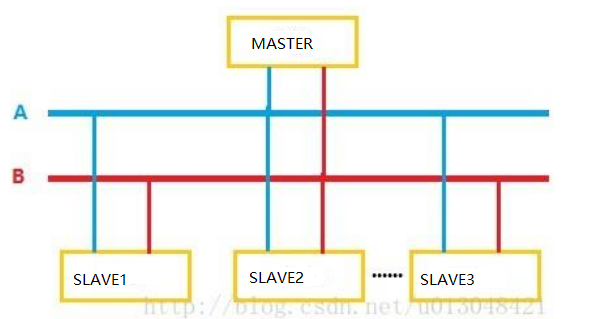
\includegraphics[width=6cm]{img/485net}
\caption{BAN }
\label{Overview}
\end{center}
\vspace{-0.5em}
\end{figure}


\end{frame}


%------------------------------------------------
\begin{frame}[fragile]{RS-485特点}

\begin{itemize}
  \item RS485通信速度快,资料最高传输速率为10Mbps以上
  \item RS485内部的物理结构,采用的是平衡驱动器和查分接收
  器的组合,抗干扰能力大大增加。
  \item  传输速率最远可达到1200米左右,使用中继可以传输更
  远距离。
\end{itemize}

\end{frame}

%------------------------------------------------
\begin{frame}[fragile]{产生时钟偏差的原因}

\begin{itemize}
  \item 初始绝对时钟不同:不同系统启动之後的初始绝对时间有
  差异
  \item 不同系统的时钟脉冲有细微差异,该差异导致绝对时钟产
  生累积误差
\end{itemize}

\end{frame}

%------------------------------------------------
\begin{frame}[fragile]{RS-485时钟同步原理-HW基础}

\begin{itemize}
  \item 如果需要MCU间的时钟同步,需要在Master和Slave之间
增加一条时钟线,Master在该时钟线上产生同步时钟方波。
\end{itemize}

\begin{figure}[htbp]
\begin{center}
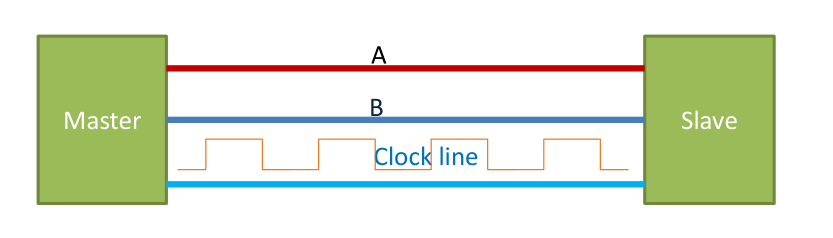
\includegraphics[width=6cm]{img/syncchart}
\caption{BAN }
\label{Overview}
\end{center}
\vspace{-0.5em}
\end{figure}
\end{frame}




%------------------------------------------------
\begin{frame}[fragile]{RS-485时钟同步原理-初始时间同步}

\begin{itemize}
  \item Master启动本地时钟,在时钟线上产生方波信号。
\item 在第一个方波信号的上升沿获取本地RTC绝对时间T 0 , 并
通过RS-485把该时间发送到Slave端
\item Slave收到方波上升沿开始计数
\item Slave收到Master发送过来的绝对时间之后,把本地RTC时间设置为T0
\end{itemize}

\begin{figure}[htbp]
\begin{center}
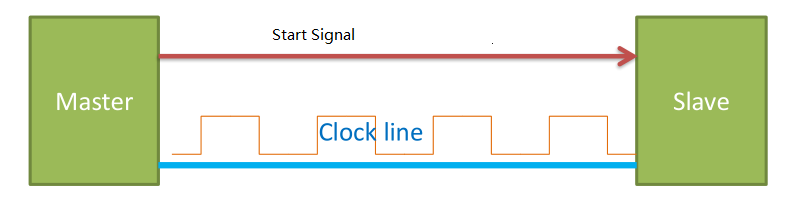
\includegraphics[width=6cm]{img/abstim}
\caption{BAN }
\label{Overview}
\end{center}
\vspace{-0.5em}
\end{figure}
\end{frame}





%------------------------------------------------
\begin{frame}[fragile]{RS-485时钟同步原理-延迟校准}
  Slave设置本地RTC绝对时间为T后,由於RS-485传输延迟和
  本地SW解析数据时间,Slave绝对时间和Master相比会有一
  定延迟,该延迟通过时钟线产生的方波进行校准,具体方法
  如下:
\begin{itemize}
  \item Slave端设置完成本地RTC绝对时间T 0 之後,等待下一次时
  钟上升沿。
\item 收到时钟上升沿之後,假设收到的是第N 0 个时钟上升沿.
重新设置本地绝对时间为:T 0 +N 0 *t. 设置完成後,Slave
绝对时间和Master绝对时间完成同步。

\end{itemize}

Note:t是时钟方波一个周期时长。


\end{frame}




%------------------------------------------------
\begin{frame}[fragile]{RS-485时钟同步原理-延迟校准}

  \begin{figure}[htbp]
  \begin{center}
  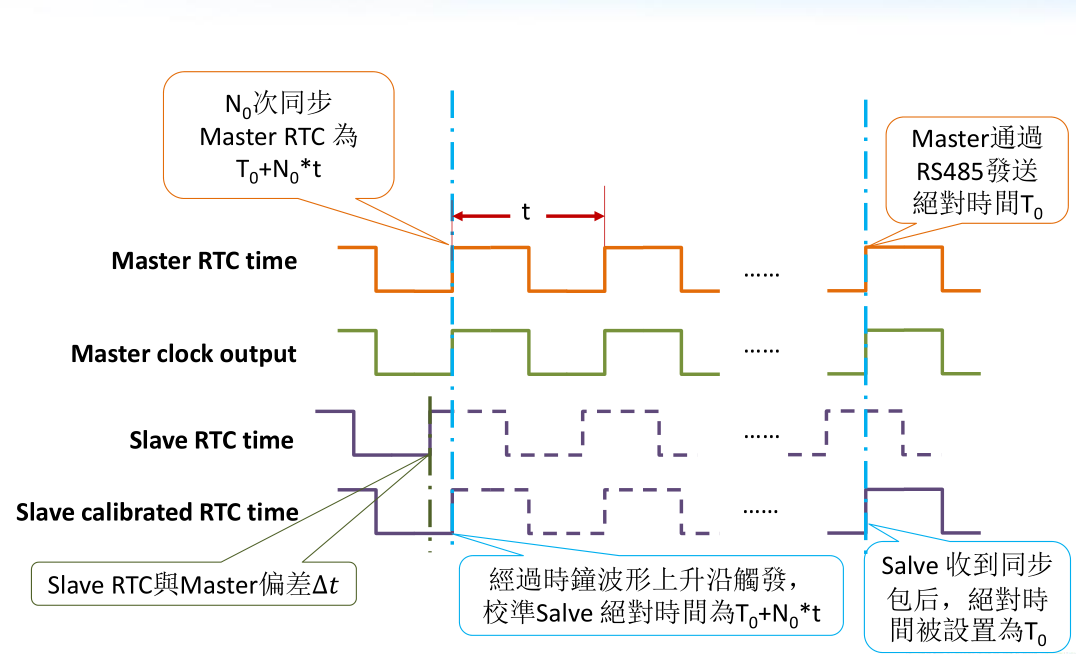
\includegraphics[width=10cm]{img/delay1}
  \caption{BAN }
  \label{Overview}
  \end{center}
  \vspace{-0.5em}
  \end{figure}

\end{frame}




%------------------------------------------------
\begin{frame}[fragile]{RS-485时钟同步原理- 时钟累积误差校准}
  Slave和Master时间完成同步后,由於两个系统有独立的时
钟脉冲,双方时钟脉冲会有误差从而导致绝对时间产生累误
差,该误差同样通过时钟方波进行校准,方法如下:


\begin{itemize}
  \item  每次Slave设置完成RTC绝对时间后,都记录该时间T并对
  方波重新计数.
\item Slave每隔N个方波都重新设置本地RTC时间为T+N*t,从
而消除累积误差。


\end{itemize}

Note:t是时钟方波一个周期时长。

\end{frame}

%------------------------------------------------
\begin{frame}[fragile]{Our Design}
我们BAN 的原本设计是这样的:
\begin{figure}[htbp]
\begin{center}
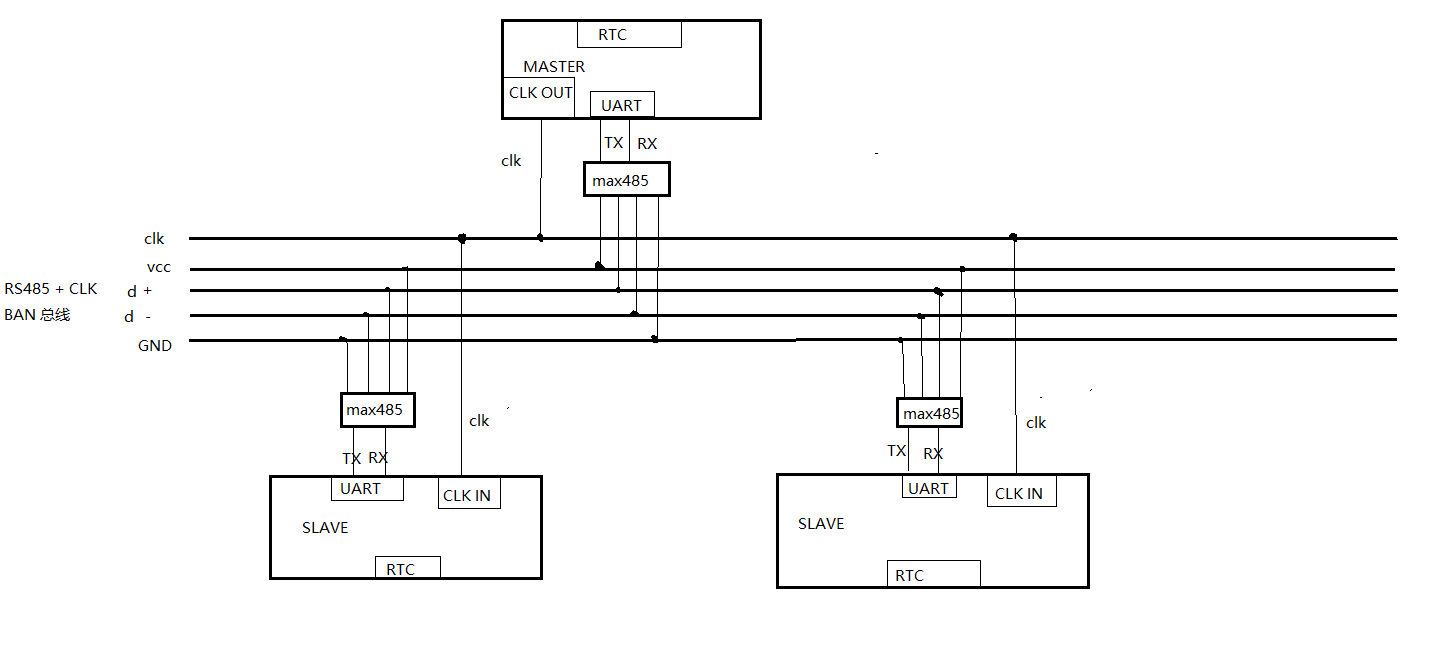
\includegraphics[width=10cm]{img/overview}
\caption{BAN }
\label{Overview}
\end{center}
\vspace{-0.5em}
\end{figure}
\end{frame}





%------------------------------------------------
\begin{frame}[fragile]{BUS}
1. 由 RS485 增添一根 clk线 形成 BAN 总线的 基本硬件线路。

2. clk 用于产生 ms 级别的脉冲波,用于时钟的同步。

3.  d+ d- 是差分处理后的数据信号。

图\ref{Overview} 假设了 挂载在总线上的设备有一个主机,两个从机。

\end{frame}

%------------------------------------------------
\begin{frame}[fragile]{UART \& 485}

max485 是一型 RS232 转 RS485 的芯片,可以把串口数据 转化为 差分信号,使其符合\textbf{RS-485}
电气规范。

STM32 方面需要实现串口的驱动,使确保串口可以实时的发送数据。接收数据。

\end{frame}

%------------------------------------------------
\begin{frame}[fragile]{RTC \& CLK}
本地时钟用于本地计数,同步时钟用于同步BAN 上设备的时钟。
\begin{itemize}
\item  RTC ,本地时钟。 每个设备都有个本地时钟。 计时粒度为 100us.

\item  CLK,同步时钟。 BAN总线上的设备使用时钟线来完成时钟同步。主设备的定时器产生同步脉冲,从设备
的定时器捕获同步脉冲完成同步。
\end{itemize}


\end{frame}


%------------------------------------------------
\begin{frame}[fragile]{Demo}

在demo 中,为了克服硬件条件的限制,我们:
\begin{itemize}
    \item 没有使用max485 来完成\textbf{TTL信号}转\textbf{差分信号}.
    \item 使用另外的一个定时器来模拟RTC的功能。
    \item 只能模拟一个主设备,一个从设备的情况。
    \item 使用串口发送开始信号
\end{itemize}

\end{frame}


%------------------------------------------------
\begin{frame}[fragile]{Demo 连线}

下图是demo 的连线和结构图:
\begin{figure}[htbp]
\begin{center}
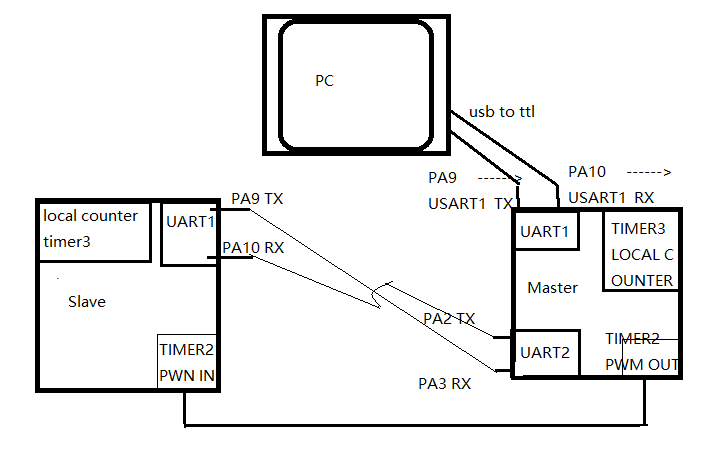
\includegraphics[width=10cm]{img/demo0}
\caption{demo}
\label{Overview}
\end{center}
\vspace{-0.5em}
\end{figure}

\end{frame}

\section{workflow}

%------------------------------------------------
%------------------------------------------------
\begin{frame}[fragile]{Demo workflow: two instructions}

\begin{enumerate}
\item Master and Slave Power on。 Peripheral Driver Initialization,Slave enters the rising edge capture state and waits for an rising edge coming.
\item When Master receives  "begin" instruction from PC.
  \begin{itemize}
    \item a.Forward to Slave first.
    \item b. start  timer3 for  MLCC(Master Local Clock Counter).
    \item c.  start timer2 to Generating Pulse Square Wave for synchronous。
  \end{itemize}
\item When Slave receives the "begin" instruction from Master, and Slave captures the first rising edge of SYNC\_CLK:
  \begin{itemize}
    \item a.  start  timer3 for  SLCC(Slave Local Clock Counter).
    \item b. Continue to capture the rising edge.

  \end{itemize}
\item "report" instructions:
\begin{itemize}
  \item a.when Master receives the "report" instruction and reports its own timestamp(MLCC) to PC.
  \item b.when Slave receives the "report" instruction, reports its own timestamp(SLCC) to Master, and Master forwards it to PC.

\end{itemize}

\end{enumerate}


\end{frame}


\begin{frame}[fragile]{Demo工作流程:两个指令}

\begin{enumerate}
\item 主机,从机上电。 外设驱动初始化。从机进入PWM 捕获状态,等待事件的发生。
\item 主机在接收到PC的 "begin"指令的时候。
  \begin{itemize}
    \item a.先转发给从机
    \item b. 开始 timer3 本地计数(local counter).
    \item c. 开始使用timer2 产生PWM 波。
  \end{itemize}
\item 当从机接收到"begin" 指令,且从机的timer2 捕获到clk上的第一个上升沿。
  \begin{itemize}
    \item a.  timer3 本地计数(local counter).
    \item b. 进入PWM 捕获同步状态。
  \end{itemize}
\item "report" 指令:
\begin{itemize}
  \item a. 主机接收到"report"指令后,上报自己的时间戳给PC。
  \item b.从机接收到"report"指令后,上报自己的时间戳给主机,主机转发给PC。
\end{itemize}

\end{enumerate}


\end{frame}




%------------------------------------------------
\begin{frame}[fragile]{定时器的应用}

主从机中:
\begin{itemize}
  \item timer2 的时钟产生或捕获PWM ,用于同步。是BAN系统中的大粒度(8ms)时钟。
  \item timer3 的时钟仅用于小粒度(100us)的 时间戳 测量。
\end{itemize}


对于从机来说,每捕获到一个上升沿 ,为了时间同步,需要强制使从机的jiffies,jiffies\_pwm增加一个捕获
周期(8ms)。


\end{frame}




%------------------------------------------------
\begin{frame}[fragile]{Demo工作流程:同步细节}

local\_tm\_t 为主从机代码中 描述时间的类型:
\begin{lstlisting}
typedef struct local_time_struct{
 unsigned char sec:7;   //秒
 unsigned char min:7;   //分
 unsigned char hour:5;  //时
 unsigned int  day;     //天
 unsigned int  jiffies; //本地时间戳
 unsigned int  jiffies_pwm;   //pwm 时间戳
} local_tm_t;
\end{lstlisting}


\begin{itemize}
  \item 主机使用timer2 产生的PWM 波 来作为同步信号,从机捕获pwm 上升沿。这个方波上升沿间隔固定且精确为4ms 或者 8ms,可以客制化,在方波的上升沿,会去触发jiffies\_pwm 累加。
  \item 主从都使用timer3 每隔100us 产生一个中断,  在中断中 jiffies 累加,到10000(1s)超时进位。作为本地时钟。
\end{itemize}

\end{frame}



%------------------------------------------------
\begin{frame}[fragile]{从机上升沿捕获中断}

tick\_sync 每隔 8ms 会被调用一次 ,用于同步本地时间戳:
\begin{lstlisting}
/* every 8ms 80*100us  */
void tick_sync(void)
{
  if( dev.local_tm.jiffies_pwm + 80 < 10000  ){
  dev.local_tm.jiffies_pwm = dev.local_tm.jiffies_pwm  + 80;
  }
  if( dev.local_tm.jiffies_pwm + 80 >= 10000  ){
    dev.evt.sec_need_update=1;
    dev.local_tm.jiffies_pwm = 80 - (10000 - dev.local_tm.jiffies_pwm);
  }
  //同步
  dev.local_tm.jiffies = dev.local_tm.jiffies_pwm;		//强等 同步
}
\end{lstlisting}

\end{frame}



%------------------------------------------------
\begin{frame}[fragile]{本地计数超时处理}

tick\_sync 每隔 100us 会被调用一次 ,用于小粒度计数:
\begin{lstlisting}
/*
  每100us 进入这个中断一次。
*/
void Tick(void)
{
  dev.local_tm.jiffies ++;
  if( dev.local_tm.jiffies % 80 == 0){
   //GPIO A5 产生 方波 用于和 同步线的方波做对比
   HAL_GPIO_WritePin(GPIOA,GPIO_PIN_5,1-HAL_GPIO_ReadPin(GPIOA,GPIO_PIN_5));
 }
  /* one second passed */
  if(dev.local_tm.jiffies >= 10000 ){
   dev.local_tm.jiffies  = 0;
 }
}
\end{lstlisting}

这里 从机的GPIOA5 有相对于 时钟同步线的方波输出。 是一个测试点。
\end{frame}





\end{document}
